\documentclass{article}
\usepackage{hyperref}
\usepackage[linguistics]{forest}
\usepackage{graphicx}
\usepackage[margin=1in]{geometry}
\usepackage{adjustbox}
\usepackage{bookmark}
\usepackage{rotating}
\usepackage{amsmath, bm, amssymb}
\usepackage{amsthm}
\usepackage{bbold}

\begin{document}
\thispagestyle{empty}
\begin{center}
    {\large\bf STAT 672}    \\*[5pt] {\Large Statistical Learning II}
    \\*[12pt] {\large John Karasev}
    \\ {\large Homework 2}
    \\ {\large January 31, 2020}
\end{center}
\section{Kernel centering}

Let $\mathcal{X}$ be a non empty set, $K$ a kernel over $\mathcal{X}$ and $H$ the 
RKHS with kernel $K$. Let $x_1,\ldots,x_n$, be $n$ points in $\mathcal{X}$.
Let $K_c$ like ``K centered\rq\rq{} be another kernel over $\mathcal{X}$ defined by 

\begin{equation}
    K_c(x,y)=\langle K(.,x)- \bar{f}(.), K(.,y)-\bar{f}(.)\rangle_H 
    \mbox{, with } \bar{f}(.)=\frac{1}{n}\sum_{i=1}^n K(.,x_i)
\end{equation}

\begin{enumerate}
    


    \item Verify that $K_c$ is a positive definite kernel; \\ 
          Let $H_c$ be the RKHS with reproducing kernel $K_c$. 

        \begin{proof}
        \begin{equation}
            \begin{aligned} 
                \mbox{for any $n$ in $\mathbb{N}$, $(a_1, ..., a_n)$ in $\mathbb{R}^n$ ,} \notag \\
                (x_1, ..., x_n) \in \mathbb{X}^n \\
                &\sum_{i,j=1}^{n} a_i a_j K_c(x_i, x_j)  \\
                &= \sum_{i,j=1}^{n} a_i a_j \langle K(.,x_i) - \bar{f}(.), K(.,x_j) - \bar{f}(.)\rangle_{\mathcal{H}} \\
                &= \bigg \langle \sum_{i=1}^{n} a_i [K(.,x_i) - \bar{f}(.)], 
                    \sum_{j=1}^{n} a_j [K(.,x_j) - \bar{f}(.)] \bigg \rangle_{\mathcal{H}} \\
                & = \bigg \| \sum_{i=1}^{n} a_i [K(.,x_i) - \bar{f}(.)] \bigg \|_{\mathcal{H}} \ge 0
            \end{aligned}
        \end{equation} 
        \end{proof}
    


    \item (**) Verify that for any $f \in H_c$, 
        
        \begin{equation}
            \frac{1}{n} \sum_{l=1}^n f(x_l)=0
        \end{equation}
        \[f(x) = \sum_{m=1}^n \alpha_m K_c(x,y_m) \notag \]
        \begin{proof}
        \begin{equation} 
            \begin{aligned} 
                \frac{1}{n} \sum_{l=1}^n f(x_l) &=0 \notag \\
                \frac{1}{n} \sum_{l=1}^n \sum_{m=1}^n \alpha_m K_c(x_l,y_m) &=0 \\
                \frac{1}{n} \sum_{l=1}^n \sum_{m=1}^n \alpha_m \bigg \langle K(.,x_l)- \frac{1}{n}\sum_{i=1}^n K(.,x_i), 
                    K(.,y_m)-\frac{1}{n}\sum_{i=1}^n K(.,x_i) \bigg \rangle_{\mathcal{H}}  &=0 \\
                \frac{1}{n} \bigg \langle \sum_{l=1}^n K(.,x_l)- \sum_{l=1}^n \frac{1}{n}\sum_{i=1}^n K(.,x_i), 
                    \sum_{m=1}^n \alpha_m K(.,y_m)-\sum_{m=1}^n \alpha_m \frac{1}{n}\sum_{i=1}^n K(.,x_i) \bigg \rangle_{\mathcal{H}}  &=0 \\
                \bigg \langle \sum_{l=1}^n K(.,x_l)- n \frac{1}{n}\sum_{i=1}^n K(.,x_i), 
                    \sum_{m=1}^n \frac{\alpha_m K(.,y_m)}{n}-\sum_{m=1}^n \frac{\alpha_m}{n}\sum_{i=1}^n \frac{K(.,x_i)}{n}  \bigg \rangle_{\mathcal{H}}  &=0 \\
                \bigg \langle 0, 
                    \sum_{m=1}^n \frac{\alpha_m K(.,y_m)}{n}-\sum_{m=1}^n \frac{\alpha_m}{n}\sum_{i=1}^n \frac{K(.,x_i)}{n}  \bigg \rangle_{\mathcal{H}}  &=0 \\
                    0&=0 \\
            \end{aligned} 
        \end{equation}
        \end{proof} 
        
        In homework 1, you have learned to sample functions from a RKHS with kernel $K$ over the set $\mathcal{X}=\{-m,\ldots,m\}$ according to the probability 
        
        \begin{equation}
            p(f)=Ce^{-\frac{||f||^2}{2}}
        \end{equation} 

        Here, you are asked to do the same thing but over the RKHS of a centered kernel $K_c$. 
        Specifically, choose  $m=10$, $n=11$, $x_1=-10,x_2=-9,\ldots,x_{11}=0$.

        \begin{equation} 
            \begin{aligned} 
                K_c(x,y) &= \bigg \langle K(.,x)- \frac{1}{n}\sum_{i=1}^n K(.,x_i), K(.,y)-\frac{1}{n}\sum_{i=1}^n K(.,x_i) \bigg \rangle \notag \\
                &= \bigg \langle K(.,x), K(.,y) \bigg \rangle + \bigg \langle K(.,x), \frac{1}{n} \sum_{i=i}^n K(.,x_i) \bigg \rangle + \\ 
                &\ \ \ \ \bigg \langle K(.,y), \frac{1}{n}\sum_{i=1}^{n} K(.,x_i) \bigg \rangle + 
                \bigg \langle \frac{1}{n} \sum_{i=1}^{n} K(.,x_i), \frac{1}{n}\sum_{j=1}^{n} K(.,x_j) \bigg \rangle \\ 
                & = K(x,y) + \frac{1}{n}\sum_{i=1}^{n}K(x,x_i) + \frac{1}{n} \sum_{i=1}^{n} K(y,x_i) + 
                \frac{1}{n^2} \sum_{i=1}^{n} \sum_{j=1}^{n} K(x_i, x_j) 
            \end{aligned} 
        \end{equation}

        % \begin{enumerate}
        %     \item[Ex. 1] 
        %         \[K_c(x,y) = e^{\frac{-(x-y)^2}{2\tau}} - \frac{1}{11}\sum_{i=-10}^{0} e^{\frac{-(x-i)^2}{2\tau}}
        %         - \frac{1}{11}\sum_{i=-10}^{0} e^{\frac{-(y-i)^2}{2\tau}} + \frac{1}{121}\sum_{i=-10}^0\sum_{j=-10}^0 e^{\frac{-(i-j)^2}{2\tau}}\]
        %     \item[Ex 2.] 
        %         \[K_c(x,y) = (x y + 600)^2 - \frac{1}{11}\sum_{i=-10}^{0} (x i + 600)^2
        %         - \frac{1}{11}\sum_{i=-10}^{0} (y i + 600)^2 + \frac{1}{121}\sum_{i=-10}^0\sum_{j=-10}^0 (i j + 600)^2\]
        %     \item[Ex. 3] 
        %         \[K_c(x,y) = tanh(xy+1) - \frac{1}{11}\sum_{i=-10}^{0} tanh(xi+1)
        %         - \frac{1}{11}\sum_{i=-10}^{0} tanh(yi+1) + \frac{1}{121}\sum_{i=-10}^0\sum_{j=-10}^0 tanh(ij+1)\]
        %     \item[Ex. 4] 
        %         \[K_c(x,y) = [xy+50] - \frac{1}{11}\sum_{i=-10}^{0} [xi+50]
        %         - \frac{1}{11}\sum_{i=-10}^{0} [yi+50] + \frac{1}{121}\sum_{i=-10}^0\sum_{j=-10}^0 [ij+50]\]
        % \end{enumerate} 

    \item (**) Write $K_c$ in term of $K$ using matrix operations. 
    
        \begin{equation} 
            \begin{aligned}
                K_c(x,y) &= K(x,y) + \frac{1}{n}\sum_{i=1}^{n}K(x,x_i) + \frac{1}{n} \sum_{i=1}^{n} K(y,x_i) + 
                \frac{1}{n^2} \sum_{i=1}^{n} \sum_{j=1}^{n} K(x_i, x_j) \notag \\
                &= K(x,y) - \frac{1}{n}\bm{K_y}^T\mathbb{1} - \frac{1}{n}\bm{K_x}^T\mathbb{1} + \frac{1}{n}\mathbb{1}^T\bm{K}\mathbb{1}
            \end{aligned}
        \end{equation}
        
        where  
        
        \[\bm{K} = [K(x_i,x_j)]_{ij\ (n,n)}\] 
        \[\bm{K_y} = [K(y,x_i)]_{i\ (1,n)}\]
        \[\bm{K_y} = [K(x,x_i)]_{i\ (1,n)}\]
        \[\mathbb{1} = [1]_{i\ (1,n)}\]
        
        The centered kernel matrix can be written as: 
        
        \begin{equation} 
            \begin{aligned}
                \bm{K_c} &= \bm{K} - \bm{UK} - \bm{KU} - \bm{UKU} \\
                &= (\bm{I} - \bm{U})\bm{K}(\bm{I-U}) \notag
            \end{aligned}
        \end{equation}

        where 
        \[\bm{U} = \bigg[\frac{1}{n}\bigg]_{ij\ (n,n)}\]
        \[\bm{I}_{\ (n,n)} \mbox{ is the indentity matrix}\]

    \item Choose the Gaussian kernel with $\tau=10$, and show 10 samples. Check that for each curve $f$, 
        
        \begin{equation}
            \frac{1}{11}\sum_{i=-10}^0 f(i)=0
        \end{equation}
        
        up to numerical errors.  

        \begin{equation} 
            \begin{aligned}
                \frac{1}{11}\sum_{i=-10}^0\bm{f}(i) = \frac{1}{11}\sum_{i=-10}^0
                    \begin{bmatrix} 
                        f_1(i) \\
                        f_2(i) \\
                        f_3(i) \\
                        \vdots \\
                        f_9(i) \\
                        f_{10}(i) 
                    \end{bmatrix}
                    = 
                    \begin{bmatrix} 
                        -0.00050791 \\
                        -0.02180374 \\
                        -0.03592173 \\
                        -0.0435211 \\
                        -0.04306572 \\
                        -0.03498534 \\
                        -0.01940224 \\
                        0.00311266 \\
                        0.03170139 \\
                        0.06432604
                    \end{bmatrix} \notag
            \end{aligned}
        \end{equation}

        \vspace{0.5cm}
        \adjustbox{valign=t}{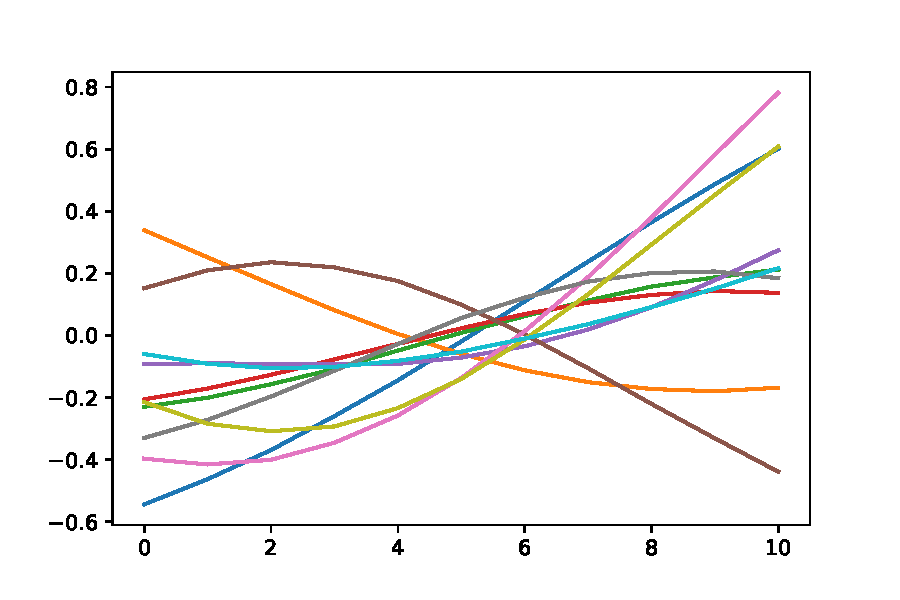
\includegraphics[width=14cm]{./figures/t10.pdf}}
        \vspace{0.5cm}

\end{enumerate}


\section{Kernel PCA}

$\mathcal{X}$ a non empty set, $x_1,\ldots,x_n \in \mathcal{X}$, $K$ a centered kernel, that is, starting with a kernel $G$ over $\mathcal{X}$, 

\[K(x,y)=\langle G(.,x)- \bar{f}, G(.,y)-\bar{f}\rangle_H \mbox{, with } \bar{f}=\frac{1}{n}\sum_{i=1}^n G(.,x_i)\]
    
Assume for simplicity that $K$ is full rank. Notate $\lambda_1 \geq \lambda_2 \geq \ldots \geq \lambda_n>0$ the e-values and $u_1,\ldots,u_n$ the corresponding e-vectors. 
We have seen in class that the principal directions $f_1,\ldots,f_n$ are 

\[f_i=\sum_{j=1}^n \alpha_{ij} K(.,x_j), \mbox{ with } \alpha_i = \lambda_i^{-\frac{1}{2}}u_i\]

\begin{enumerate}

    \item verify that \[\langle f_i,f_k \rangle_H=\delta_{ik}\]
    where $\delta_{ik}=1$ if $i=k$ and $\delta_{ik}=0$ if $i \not = k$. 

    \begin{equation} 
        \begin{aligned}
            \langle f_i, f_k \rangle_{\mathcal{H}} &= \lambda^{-\frac{1}{2}}_i \bm{u}_i^T\bm{K}\bm{u}_k \lambda_k^{-\frac{1}{2}} \notag 
            = \lambda^{-\frac{1}{2}}_i \bm{u}_i^T\bm{U \Lambda U}^T\bm{u}_k \lambda_k^{-\frac{1}{2}} \\
            &= \lambda^{-\frac{1}{2}}_i \bm{e}_i^T\bm{\Lambda}\bm{e}_k \lambda_k^{-\frac{1}{2}} 
            = \lambda^{-\frac{1}{2}}_i \lambda_i\bm{e}_i^T\bm{e}_k \lambda_k^{-\frac{1}{2}} 
            = \frac{\lambda^{\frac{1}{2}}_i}{\lambda_k^{-\frac{1}{2}}} \bm{e}_i^T\bm{e}_k \\
            &= 
                \begin{cases} 
                    0 \mbox{, if $i \ne j$} \\
                    1 \mbox{, else}
                \end{cases} 
            = \delta_{ik}
        \end{aligned}
    \end{equation}
    where \[e_k = [1\ if\ k=j\ else\ 0]_{(j,1)}\]
    
    \item Show that the orthogonal projection of any $f \in H$, the RKHS with kernel $K$ onto 
        
        \[V=span\{f_1,\ldots,f_n\}\]

        is

        \[\pi_v(f)=\langle f,f_1\rangle_H f_1+\ldots,\langle f,f_n\rangle_H f_n\]

        Now, let us project the feature functions of $x_1,\ldots,x_n$, that is $K(.,x_1), \ldots K(.,x_n)$. Show that 

        \[\langle K(.,x_k),f_i \rangle = \lambda_i^\frac{1}{2} u_{ki}\]
    
    \item Perform kernel PCA on the MNIST dataset. Choose the digits 1 and 7. 
    Start with the linear kernel $G(x,y)=x^Ty$. Sample $n=500$ digits. Show 8 
    projections onto the first 8 principal directions. Do not forget to center the 
    kernel. 


    \item Redo the same but this time with a non linear kernel of your choice.  
    
%     &\ \ e_k^T K u_i \lambda_i^{-\frac{1}{2}} \\
% &= e_k^T U \Lambda U^T u_i \lambda_i^{-\frac{1}{2}} \\
% &= e_k^T U \Lambda e_i \lambda_i^{-\frac{1}{2}} = e_k^T U e_i \lambda_i^{\frac{1}{2}} \\
% & = e_k^T u_i \lambda_i^{\frac{1}{2}} = u_{i}[k] \lambda_i^{\frac{1}{2}}
    
    

\end{enumerate}

\end{document}
